
\newcommand{\PaperTitleMapping}{Nonlinear grid mapping applied to an FDTD-based, multi-center 3D
                                  Schr\"odinger equation solver}

\section{\PaperTitleMapping}
\label{section:papers:qfdtd}

\begin{flushright}
Nicolas Bigaouette, Edward Ackad, Lora Ramunno
\end{flushright}

% Include PDF's abstract in the Table-of-Content as ``subsection 0'' but hide the number
\HidePDFAbstractNumber

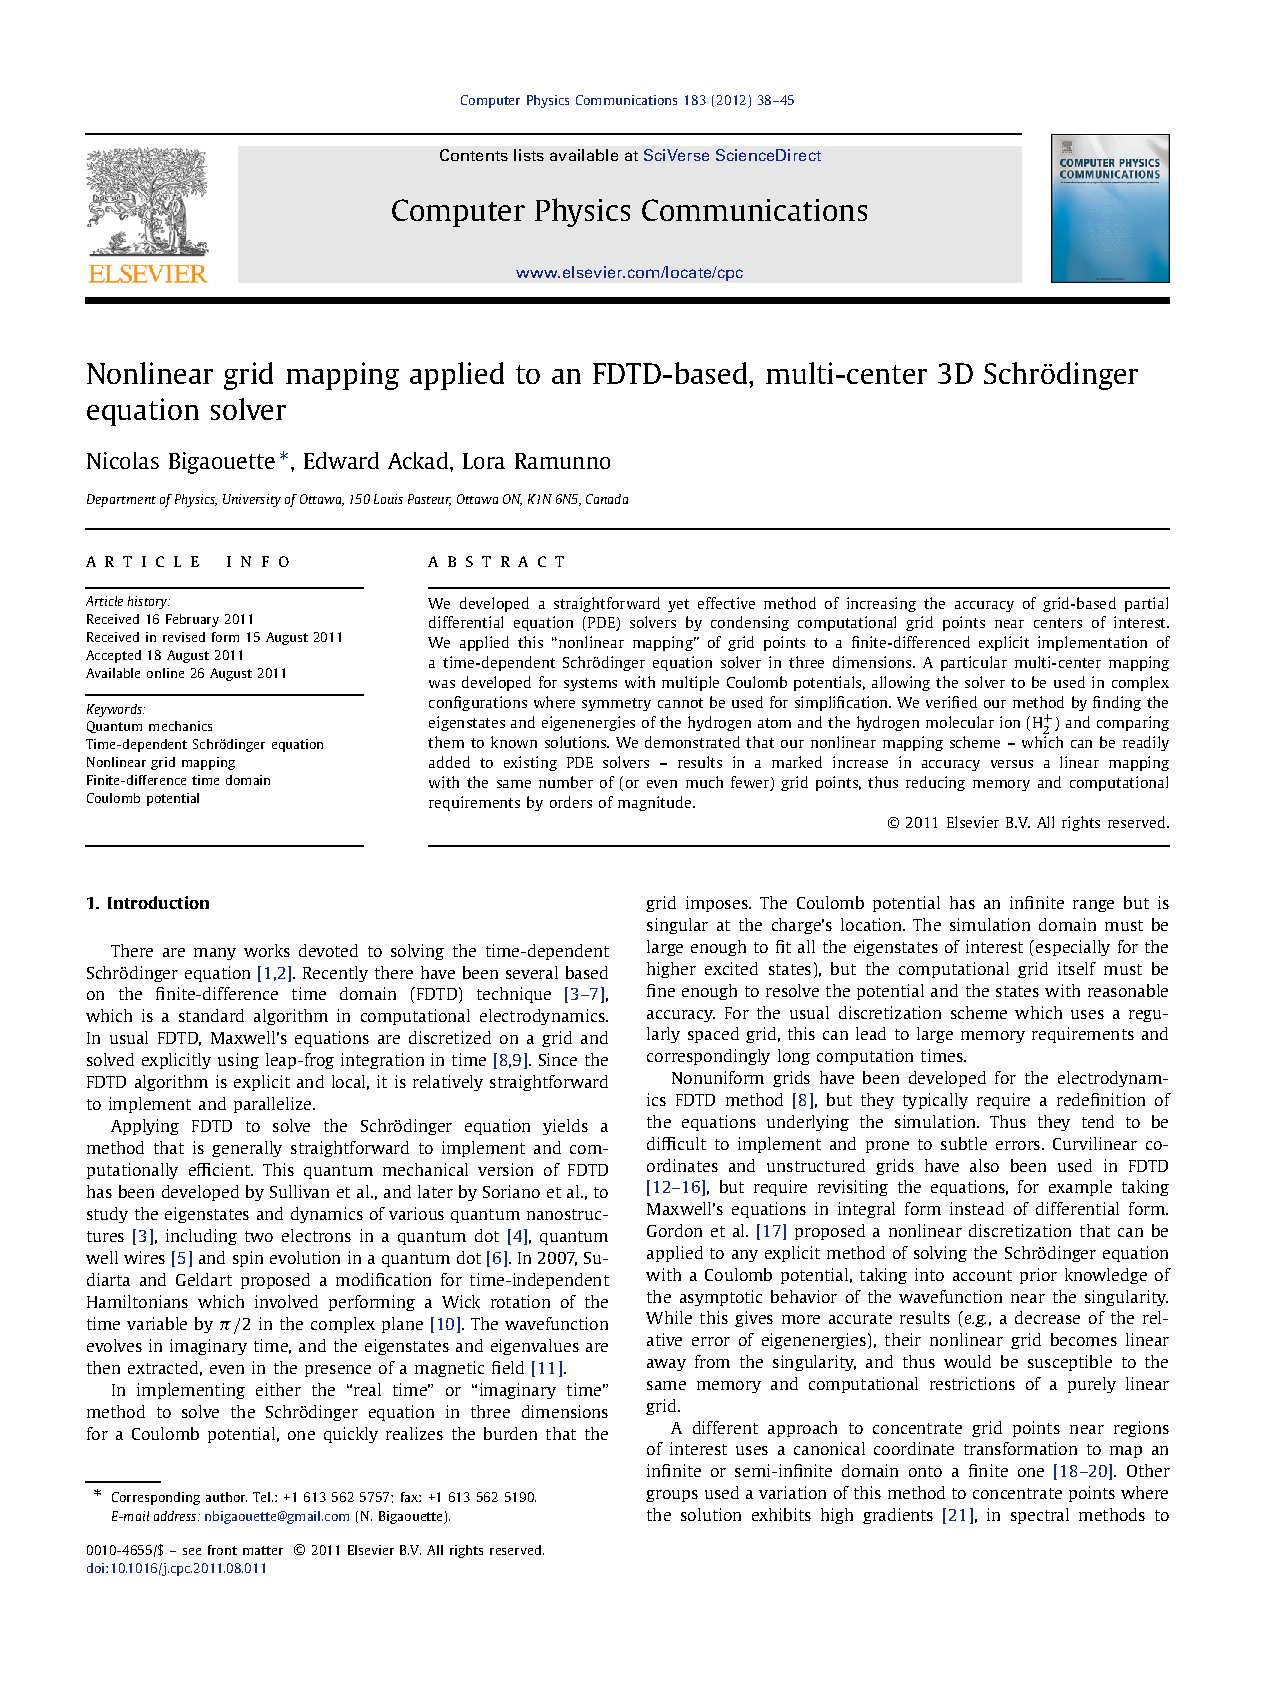
\includepdf[pages=-,
            addtotoc={
                %1,section,1,\PaperTitleMapping,paper_mapping,
                1,subsection,2,Abstract,paper_mapping_Abstract,
                1,subsection,2,Introduction,paper_mapping_intro,
                2,subsection,2,Finite-differenced Schrödinger equation,paper_mapping_fdtd,
                2,subsubsection,3,Real-time,paper_mapping_realtime,
                3,subsubsection,3,Imaginary-time,paper_mapping_imagtime,
                3,subsection,2,Details of nonlinear mapping,paper_mapping_details,
                4,subsubsection,3,General approach,paper_mapping_details_general,
                4,subsubsection,3,Details of the implementation,paper_mapping_details_details,
                5,subsubsection,3,Nonlinear mapping for the Coulomb potential,paper_mapping_details_coulomb,
                6,subsection,2,Validation and results,paper_mapping_results,
                6,subsubsection,3,Hydrogen atom,paper_mapping_results_h,
                7,subsubsection,3,Hydrogen cation molecule,paper_mapping_results_h2p,
                7,subsection,2,Conclusion,paper_mapping_conclusion,
                8,subsection,2,References,paper_mapping_ref
            }]{papers/Bigaouette2011_Mapping.pdf}
